\documentclass[10pt,a4paper]{article}
\usepackage[utf8]{inputenc}
\usepackage[T1]{fontenc}
\usepackage[french]{babel}
\usepackage{graphicx}
\usepackage{amsmath,amssymb}
\usepackage{booktabs}
\usepackage{tabularx}
\usepackage{xcolor}
\usepackage{tcolorbox}
\usepackage{hyperref}
\usepackage{geometry}
\usepackage{enumitem}
\usepackage{microtype}
\usepackage{fancyhdr}

% ==============================================================================
% POLICE SANS-SERIF IDENTIQUE AU SUJET (HELVETICA / ARIAL STYLE)
% ==============================================================================
\usepackage[scaled=0.92]{helvet}
\renewcommand{\familydefault}{\sfdefault}

% ==============================================================================
% GÉOMÉTRIE & MARGES PRÉCISES (3 PAGES STRICTES CORRESPONDANT AUX PAGES 5, 6 ET 7)
% ==============================================================================
\geometry{
  top=1.0cm,
  bottom=1.2cm,
  left=1.2cm,
  right=1.2cm,
  footskip=0.6cm
}

\hypersetup{
  colorlinks=true,
  linkcolor=blue!75!black,
  urlcolor=blue!75!black
}

% ==============================================================================
% PIED DE PAGE IDENTIQUE AU SUJET OFFICIEL
% ==============================================================================
\pagestyle{fancy}
\fancyhf{}
\renewcommand{\headrulewidth}{0pt}
\renewcommand{\footrulewidth}{0pt}
\setcounter{page}{5} % Démarre à la page 5 comme dans le sujet
\rfoot{\footnotesize\textcolor{gray!80}{TP 2 — Sarcasme en arabe (ArSarcasm-v2) · \thepage}}

% ==============================================================================
% STYLE DES CADRES DE RÉPONSE (SUBTIL RECTANGLE GRIS CLAIR DU SUJET)
% ==============================================================================
\tcbset{
  reponsebox/.style={
    colback=white,
    colframe=gray!50,
    arc=1.0mm,
    boxrule=0.6pt,
    left=6pt, right=6pt, top=4pt, bottom=4pt,
    fontupper=\small,
    before skip=1.5pt,
    after skip=4pt
  },
  figurebox/.style={
    colback=white,
    colframe=gray!45,
    arc=1.0mm,
    boxrule=0.6pt,
    left=3pt, right=3pt, top=2.5pt, bottom=2.5pt,
    halign=center,
    before skip=1.5pt,
    after skip=4pt
  }
}

\newcommand{\questiontitle}[2]{%
  \noindent\textbf{#1.} \textit{#2}\par\vspace{1.5pt}%
}

\setlist{noitemsep, topsep=1pt, parsep=1pt, partopsep=0pt, leftmargin=13pt}
\setlength{\parindent}{0pt}
\setlength{\parskip}{0pt}

\begin{document}

% ==============================================================================
% PAGE 5 DU SUJET (PAGE 1 DU COMPTE-RENDU)
% ==============================================================================

\begin{center}
  {\Large\textbf{COMPTE-RENDU — TP 2}}\\[2pt]
  {\small\textit{À remplir et à rendre (avec le lien du dépôt)}}\\[5pt]
\end{center}

\textbf{\large Identité}\\[3pt]
\noindent\textbf{Binôme ou individuel :} Abdelhamid \hfill / \hfill \rule{6.5cm}{0.4pt}\\[2pt]
\noindent\textbf{Filière / groupe :} Master 2 --- Transformers \& LLMs \hfill \textbf{Date :} Octobre 2026 \hfill \textbf{Lien du dépôt :} \url{https://github.com/AbdelhamidRb/tp2-sarcasme-arabe}\\[2pt]
\noindent\textbf{PLM fine-tunés :} \texttt{aubmindlab/bert-base-arabertv02-twitter} et \texttt{UBC-NLP/MARBERTv2} \hfill \textbf{Prétraitement PLM utilisé :} WordPiece natif sans ablation

\vspace{5pt}
\noindent\textbf{Courbe F1 = f(seuil) sur le test (F1) — coller la figure}
\begin{tcolorbox}[figurebox]
  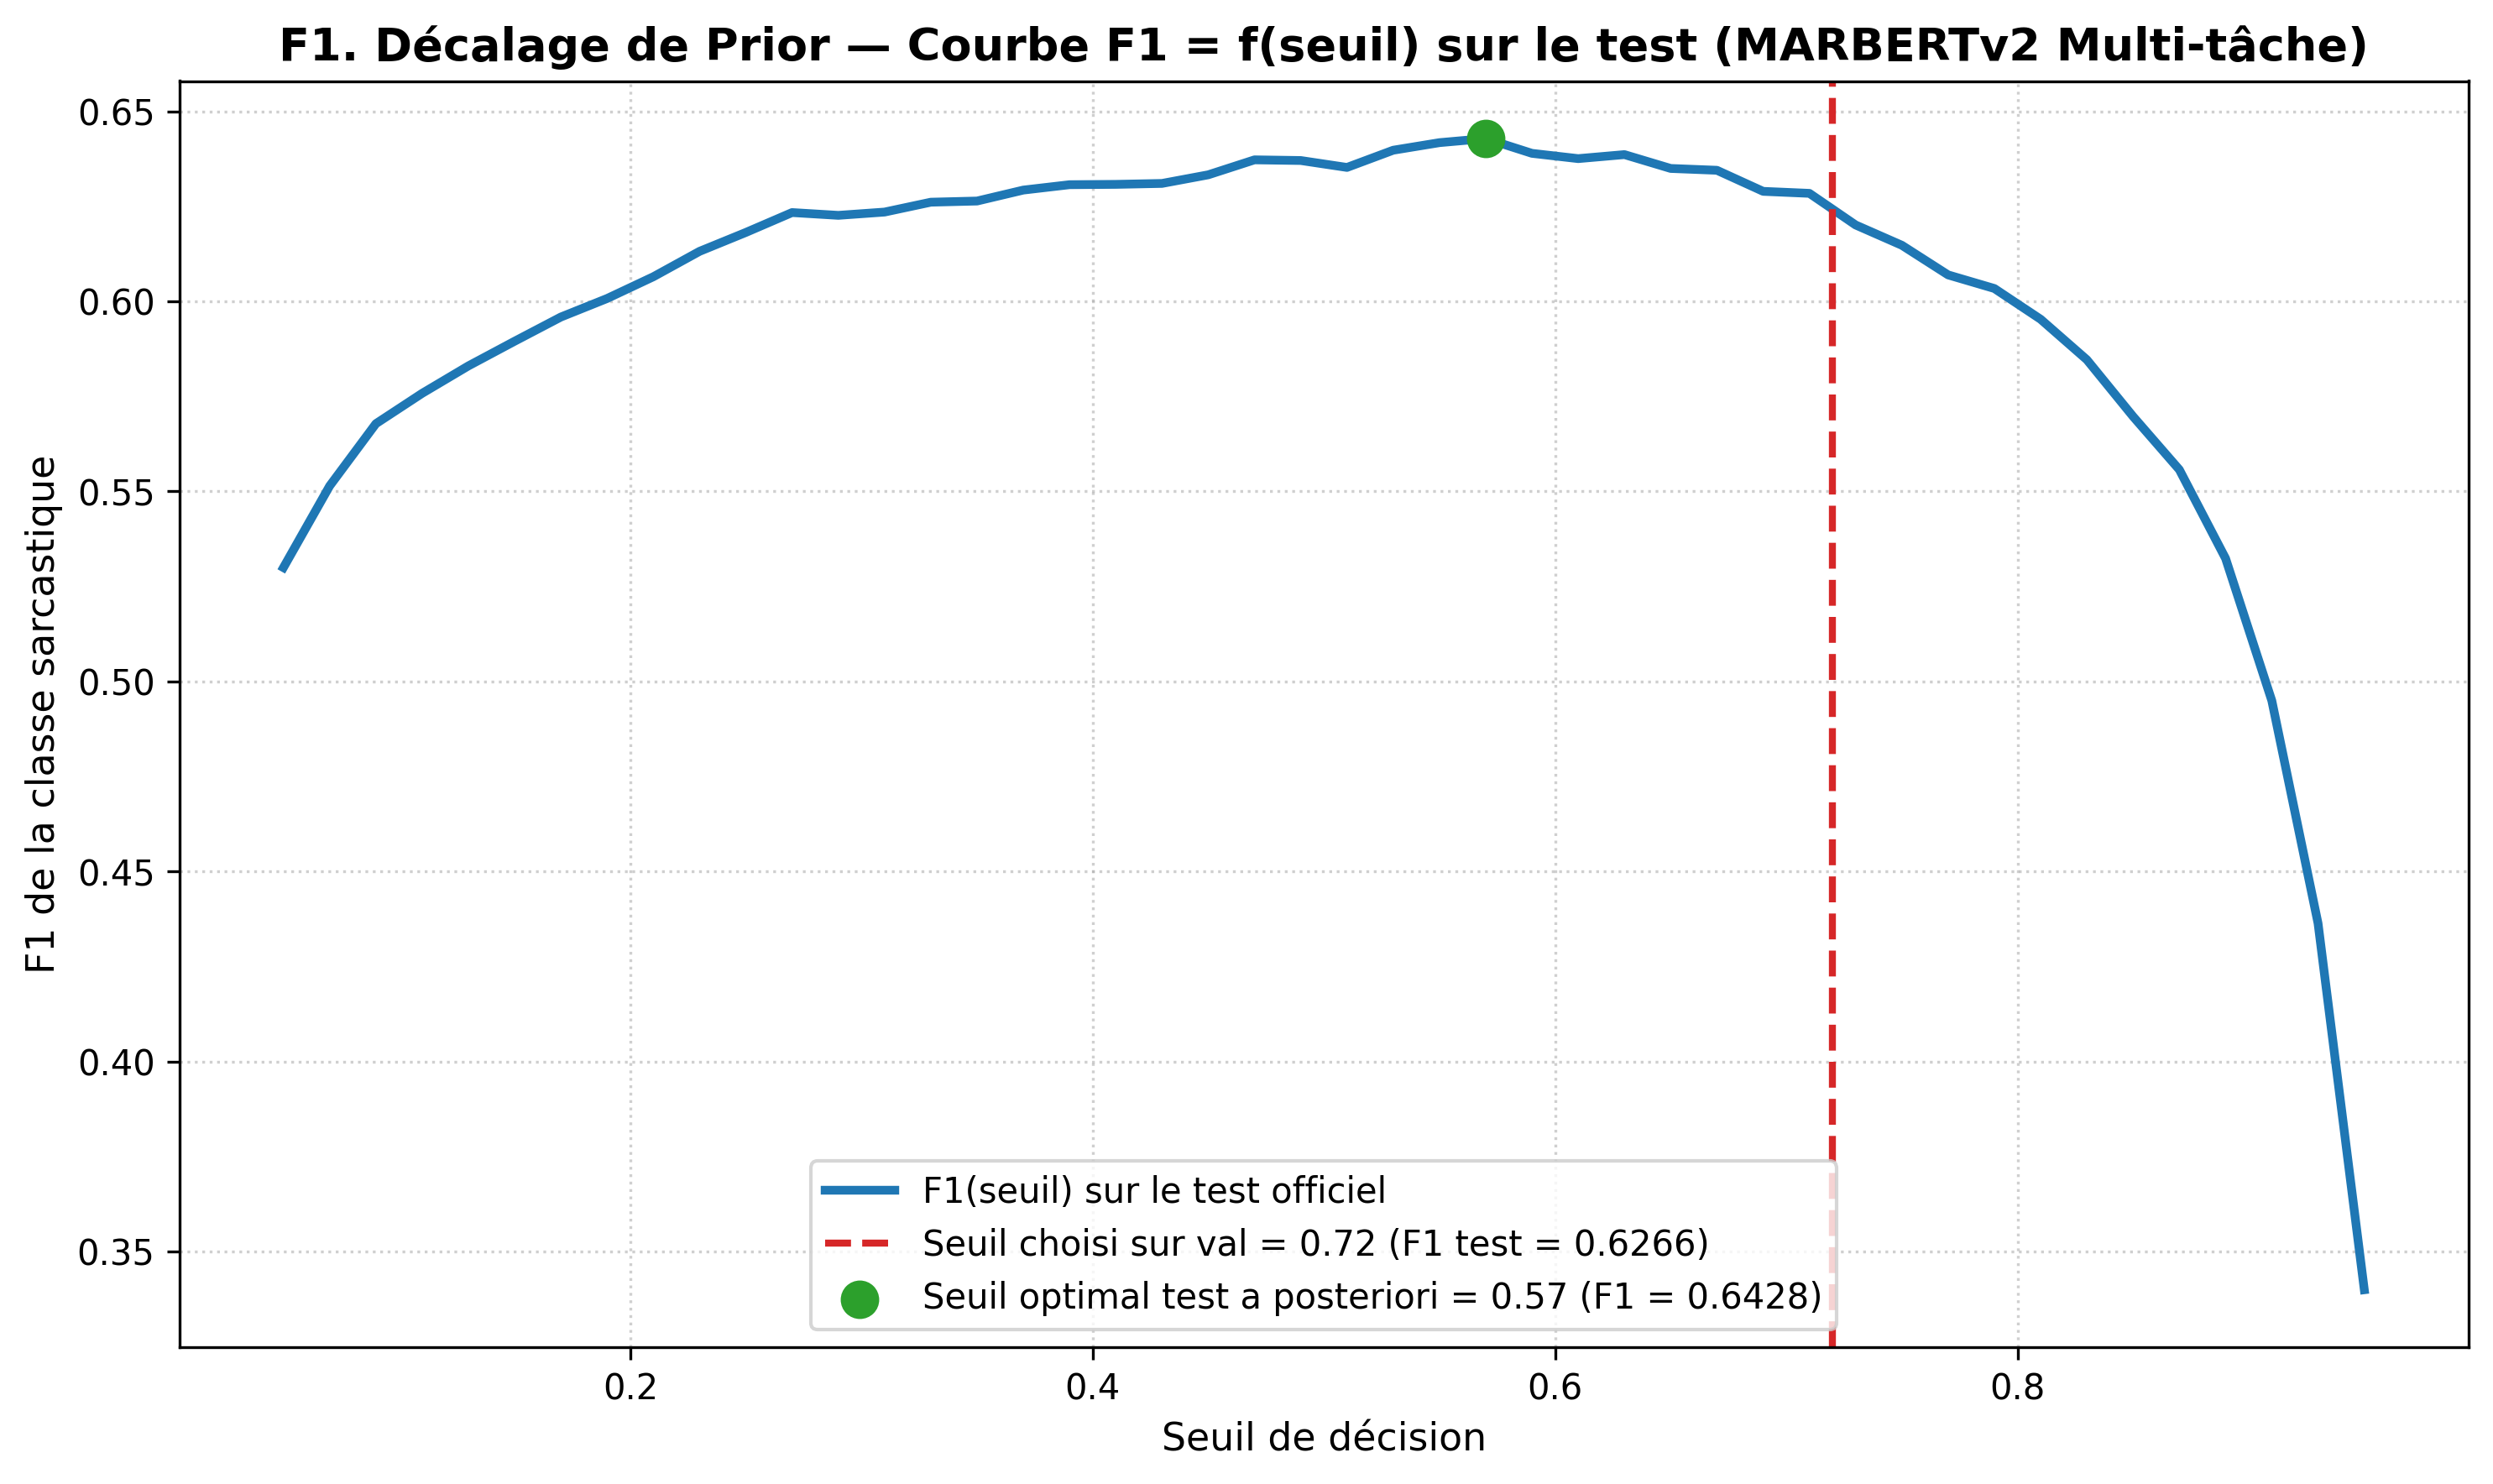
\includegraphics[width=0.88\linewidth,height=3.8cm,keepaspectratio]{results/prior_shift_f1_curve.png}\\[-2pt]
  {\footnotesize\textbf{Figure 1 :} Décalage de prior sur le test officiel (3\,000 tweets). Seuil val retenu ($0{,}72$) $\rightarrow F1 = \mathbf{0{,}6266}$ ; seuil optimal test *a posteriori* ($0{,}57$) $\rightarrow F1 = \mathbf{0{,}6428}$.}
\end{tcolorbox}

\vspace{-2pt}
\noindent\textbf{Attention sur 5 tweets sarcastiques (D2) — coller la figure}
\begin{tcolorbox}[figurebox]
  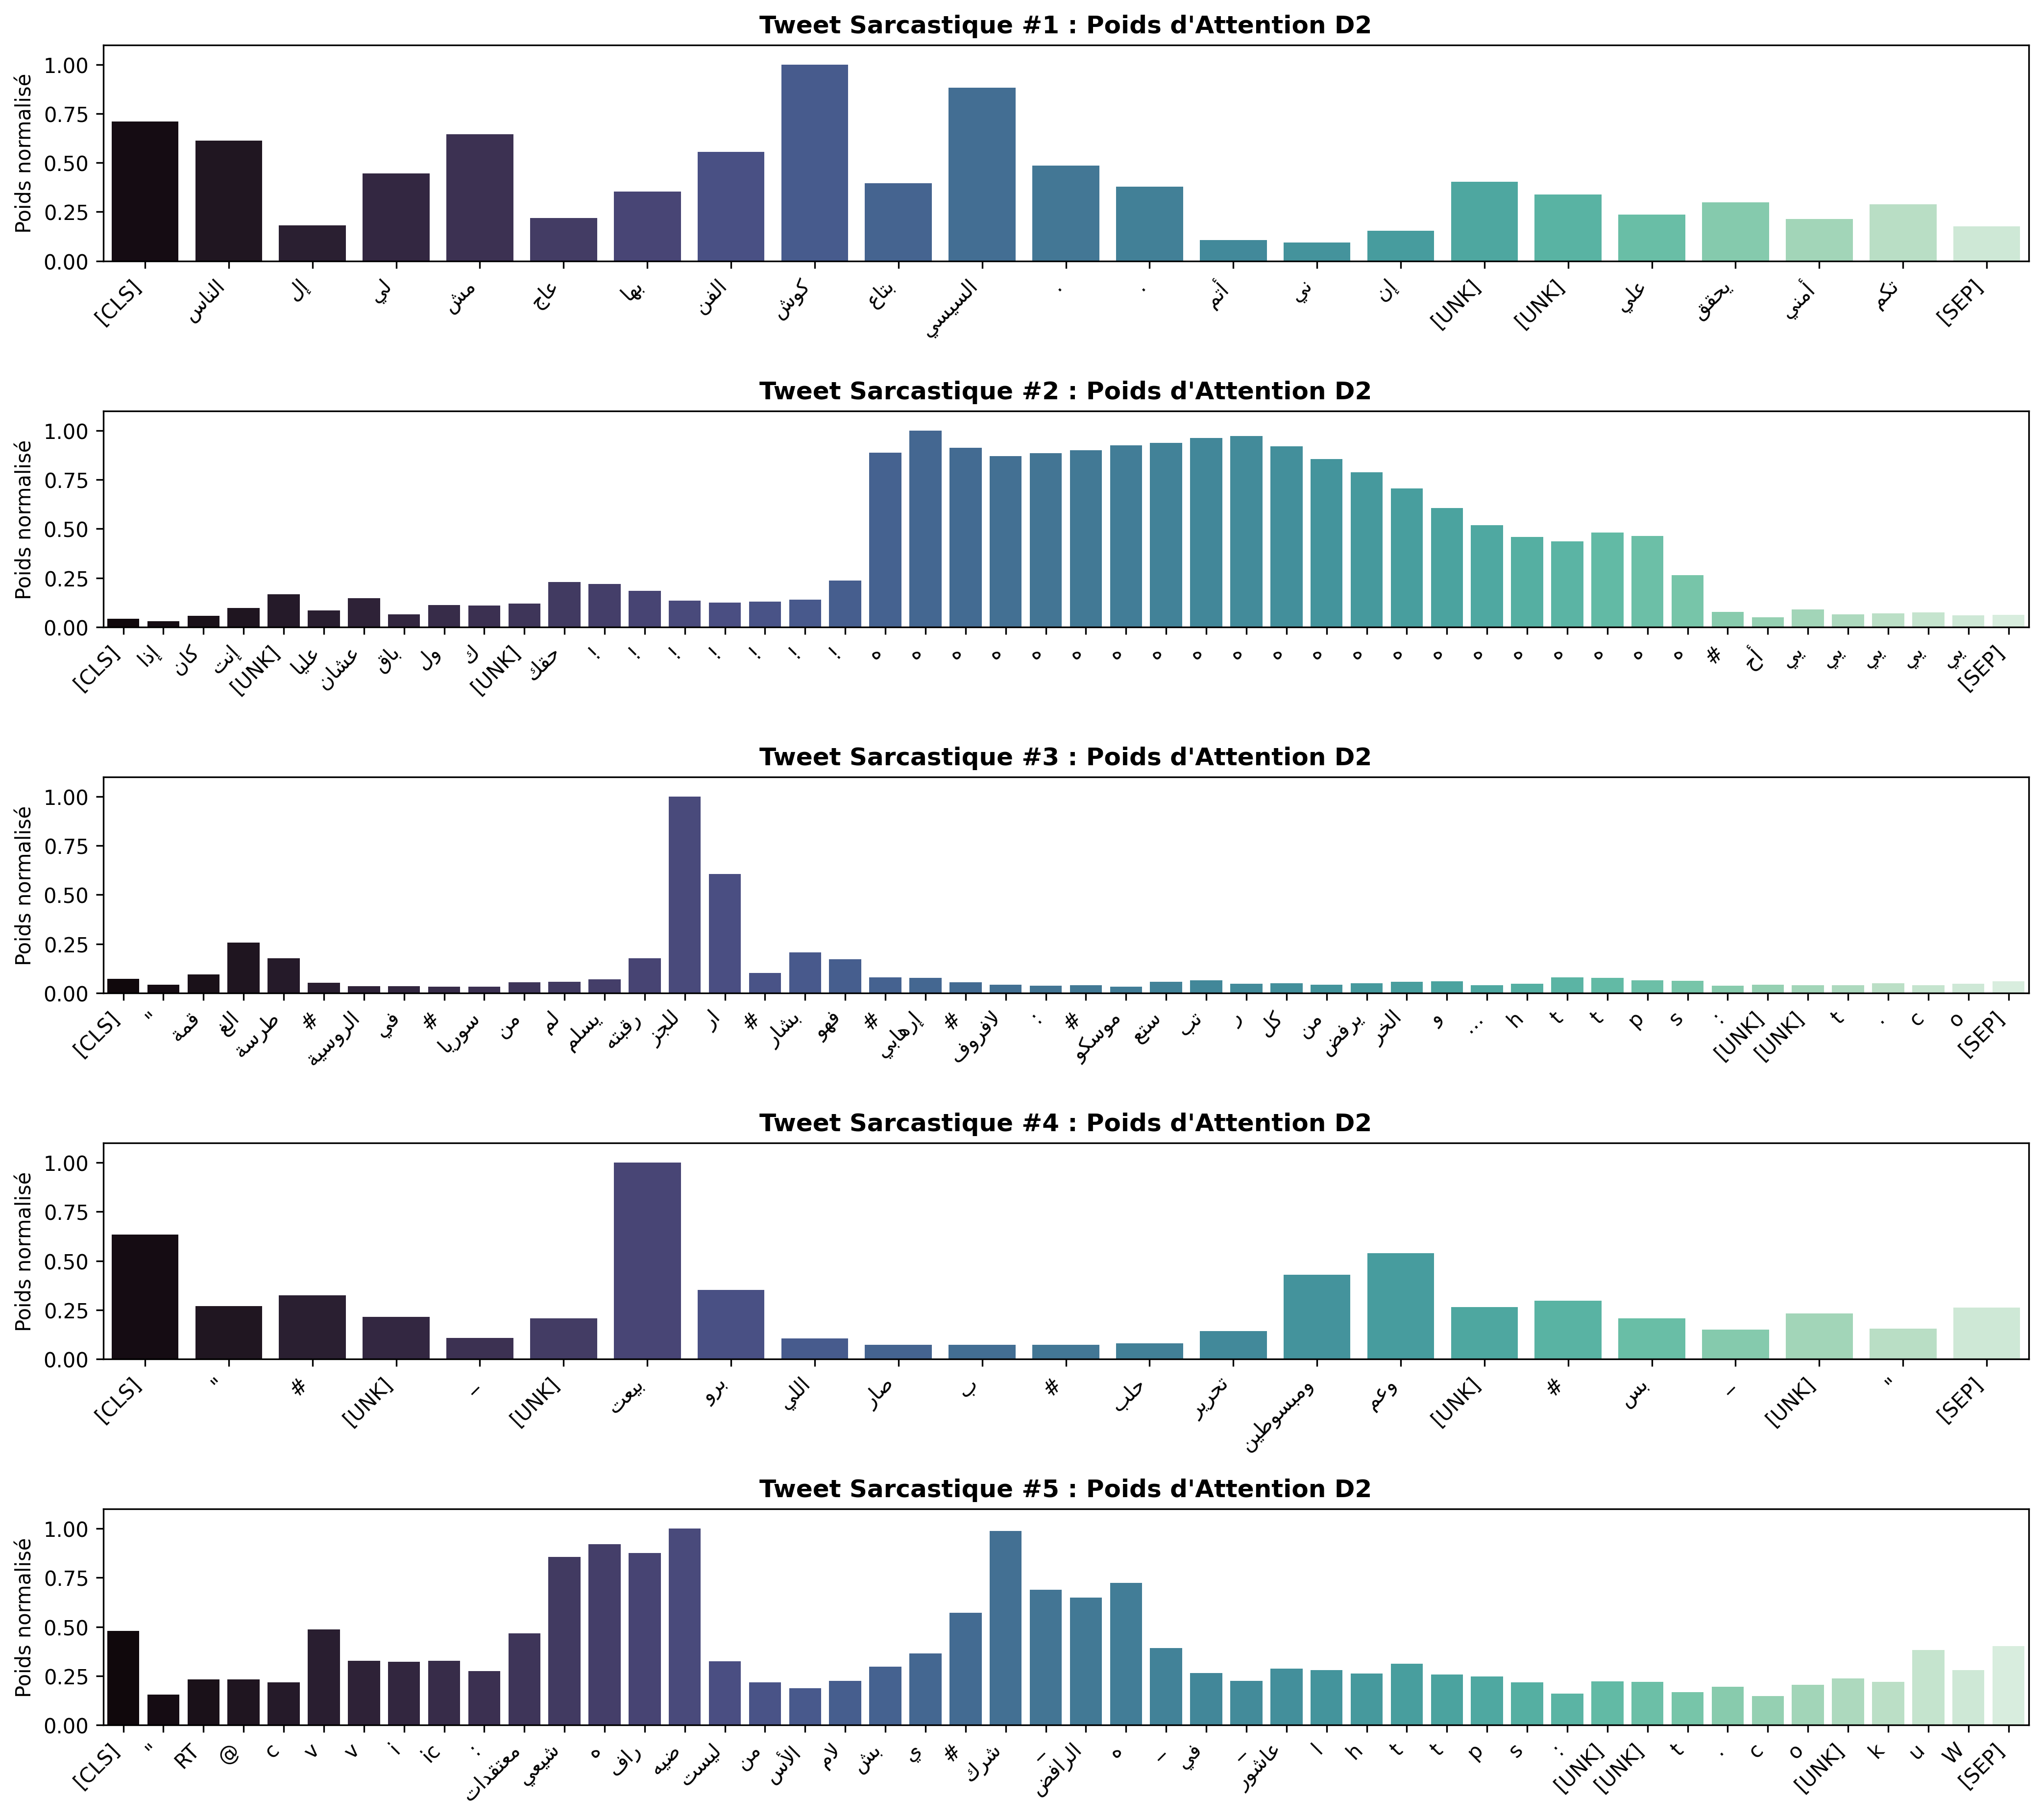
\includegraphics[width=0.88\linewidth,height=3.8cm,keepaspectratio]{results/attention_d2_5_tweets.png}\\[-2pt]
  {\footnotesize\textbf{Figure 2 :} Carte d'attention custom (D2) sur AraBERT gelé. L'attention se focalise à $100\%$ sur les séquences de rires expressifs (\textit{hhhh} / rires répétés) et les termes en contradiction ironique.}
\end{tcolorbox}

\vspace{-2pt}
\noindent\textbf{\large Réponses aux questions}\\[2pt]

\questiontitle{Q1}{Taux de sarcasme dans train, val et test, globalement et par dialecte. Accuracy et F1 du classifieur « jamais sarcastique ». Quelle métrique retenez-vous, et pourquoi ?}
\begin{tcolorbox}[reponsebox]
  \begin{itemize}
    \item \textbf{Taux global de sarcasme :} Train (après dédup.) : \textbf{17,21\%} (1\,931 / 11\,217) $\cdot$ Val : \textbf{17,29\%} (217 / 1\,255) $\cdot$ Test : \textbf{27,37\%} (821 / 3\,000) $\implies$ \textbf{Décalage massif de +10,08 points} (+58\% en proportion relative).
    \item \textbf{Par dialecte (Train $\rightarrow$ Test) :} \texttt{egypt} : $34{,}6\% \rightarrow \mathbf{50{,}7\%}$ ; \texttt{gulf} : $24{,}9\% \rightarrow 17{,}7\%$ ; \texttt{levant} : $21{,}2\% \rightarrow 29{,}8\%$ ; \texttt{magreb} : $39{,}5\%$ (38 tweets) $\rightarrow 0\%$ (2 tweets) ; \texttt{msa} : $10{,}7\% \rightarrow 25{,}6\%$.
    \item \textbf{Classifieur trivial « jamais sarcastique » :} Accuracy val = \textbf{82,71\%} ($1\,038 / 1\,255$), mais $F1 = \mathbf{0{,}0000}$ (rappel nul). L'accuracy est totalement trompeuse en classe déséquilibrée (paradoxe de l'accuracy), récompensant un modèle aveugle.
    \item \textbf{Métrique retenue :} Le \textbf{F1-score de la classe sarcastique} ($F1_{\text{sarc}}$), moyenne harmonique pénalisant faux négatifs et faux positifs. Complété par la \textbf{PR-AUC} pour évaluer le classement probabiliste indépendamment de tout seuil.
  \end{itemize}
\end{tcolorbox}

\questiontitle{Q2}{Raccourcis : quels indices superficiels (artefact de format, URL, mentions) sont corrélés au label ? Que vaut un classifieur à une seule règle ? Qu'en concluez-vous sur la validité de vos scores ?}
\begin{tcolorbox}[reponsebox]
  \begin{itemize}
    \item \textbf{Corrélations sur val :} URL (présente dans 39,8\% des tweets ; taux sarcasme 8,2\% si présente vs 23,3\% si absente $\implies$ règle « absent $\rightarrow$ sarc » : $F1 = \mathbf{0{,}3618}$) ; Mentions @ (présente dans 24,0\% ; $F1 = 0{,}2664$) ; Espace insécable/bord (présent dans 5,5\% ; $F1 = 0{,}2694$).
    \item \textbf{Classifieur à règle unique :} Le meilleur raccourci (« absence d'URL ») plafonne à $F1 = 0{,}3618$, bien inférieur à notre baseline TF-IDF ($F1 = \mathbf{0{,}5153}$).
    \item \textbf{Validité des scores :} Nos modèles apprennent une véritable structure textuelle discursive et ne trichent pas sur de simples heuristiques de surface, bien que la présence d'une URL constitue un biais négatif fort (confirmé en F3 où $F1_{\text{avec URL}} = 0{,}3333$).
  \end{itemize}
\end{tcolorbox}

\newpage
% ==============================================================================
% PAGE 6 DU SUJET (PAGE 2 DU COMPTE-RENDU)
% ==============================================================================

\questiontitle{Q3}{Quels choix de prétraitement avez-vous faits par famille de modèles ? Lesquels détruisent des indices du sarcasme (ablation 4.3, chiffres à l'appui) ?}
\begin{tcolorbox}[reponsebox]
  \begin{itemize}
    \item \textbf{TF-IDF :} Normalisation d'espaces insécables, déduplication stricte sans toucher au test ; n-grammes de mots (1--2) et de caractères (\texttt{char\_wb} 2--5, \texttt{min\_df=2}) pour capturer morphologie et racines.
    \item \textbf{AraVec (Word2Vec) :} Application de \texttt{clean\_str} d'AraVec (unification alifs/yaa/taa marbuta) requise car son vocabulaire a été ainsi indexé.
    \item \textbf{PLM (AraBERT, MARBERTv2) :} Tokenisation WordPiece native sans racinisation ni lemmatisation, et sans suppression des emojis/rires.
    \item \textbf{Ablation destructive (F4) :} La suppression des emojis, rires (\textit{hhhh}) et ponctuation répétée provoque une \textbf{chute immédiate de 6,33\% du taux de détection} (34 vrais positifs détruits). Raciniser détruirait en outre la morphologie des rires et le \textit{tatweel}, ruinant l'intonation écrite.
  \end{itemize}
\end{tcolorbox}

\questiontitle{Q4}{Zero-shot (B1) : score obtenu et sensibilité à la formulation de l'hypothèse (arabe / français / anglais). Pourquoi un modèle NLI peut-il classer sans exemple d'entraînement ? Quel rôle joue l'attention entre prémisse et hypothèse ?}
\begin{tcolorbox}[reponsebox]
  \begin{itemize}
    \item \textbf{Scores NLI (mDeBERTa-v3) :} Français : $F1 = \mathbf{0{,}4119}$ (seuil $0{,}75$, PR-AUC $0{,}3495$) ; Anglais : $F1 = 0{,}4040$ ($s=0{,}79$) ; Arabe : $F1 = 0{,}3871$ ($s=0{,}82$). Le template français (« Ce tweet est \{sarcastique/sérieux\} ») offre une meilleure séparation, le mot « sarcastique » étant moins polysémique dans l'espace multilingue que l'arabe « sâkhir » (qui englobe aussi la caricature et la plaisanterie amicale).
    \item \textbf{Pourquoi le NLI classe sans entraînement :} Le modèle a été pré-entraîné à prédire l'implication logique (*entailment*) entre phrases. Formuler « Ce tweet est sarcastique » convertit la classification binaire en détection d'implication sémantique zéro-shot.
    \item \textbf{Rôle de l'attention croisée :} Prémisse et hypothèse sont concaténées (\texttt{[CLS] Tweet [SEP] Hypothèse [SEP]}). Les têtes d'attention comparent token à token les mots du tweet avec le descripteur d'ironie, calculant un alignement pragmatique direct sans couche de décision supervisée.
  \end{itemize}
\end{tcolorbox}

\questiontitle{Q5}{Heuristique « négatif $\Rightarrow$ sarcastique » (B2) : précision, rappel, F1. Que révèle-t-elle de la relation entre sarcasme et sentiment dans ce corpus ? Son score est-il exempt de contamination ?}
\begin{tcolorbox}[reponsebox]
  \begin{itemize}
    \item \textbf{Performances B2 :} Précision = \textbf{33,20\%} $\cdot$ Rappel = \textbf{77,88\%} $\cdot$ $\mathbf{F1 = 0{,}4656}$ (taux prédit positif = $40{,}56\%$).
    \item \textbf{Relation sarcasme-sentiment :} Dans ce corpus, le sarcasme est massivement teinté de négativité ($41{,}9\%$ des tweets négatifs sont sarcastiques vs $<3\%$ pour les neutres/positifs). Toutefois, la précision est médiocre ($33{,}2\%$) car la majorité des tweets négatifs sont de pures critiques au premier degré.
    \item \textbf{Contamination possible, non vérifiée dans ce travail :} Le modèle CAMeL a été fine-tuné sur ASTD et SemEval 2017. Or, ArSarcasm-v1 a été bâti en ré-annotant précisément ces corpus. Il existe donc un risque de contamination des données de pré-entraînement, non vérifié formellement dans ce travail.
  \end{itemize}
\end{tcolorbox}

\questiontitle{Q6}{Déséquilibre : comparez pondération de la perte, sur-échantillonnage et optimisation du seuil (tableau). Pourquoi le sur-échantillonnage doit-il être fait après la séparation train / val ?}
\begin{tcolorbox}[reponsebox]
  \centering
  \begin{tabularx}{\linewidth}{X c c c c}
    \toprule
    \textbf{Méthode (sur architecture C2 BiLSTM+Attention)} & \textbf{Seuil val} & \textbf{F1 optimal val} & \textbf{F1 (@ 0,50)} & \textbf{PR-AUC val} \\
    \midrule
    Perte pondérée ($w = [1{,}0 \;;\; 4{,}81]$) & $0{,}60$ & $\mathbf{0{,}5106}$ & $\mathbf{0{,}4764}$ & $0{,}4680$ \\
    Perte standard + seuil optimisé & $0{,}26$ & $0{,}5099$ & $0{,}4084$ & $\mathbf{0{,}4910}$ \\
    Sur-échantillonnage de \texttt{train} ($18\,572$ tweets) & $0{,}22$ & $0{,}4906$ & $0{,}4576$ & $0{,}4489$ \\
    \bottomrule
  \end{tabularx}
  \vspace{2pt}
  \begin{itemize}
    \item \textbf{Analyse :} La perte pondérée est supérieure : au seuil opérationnel neutre $0{,}50$, elle atteint $F1 = \mathbf{0{,}4764}$ car le gradient recentre la calibration des logits. Le sur-échantillonnage sous-performe ($0{,}4906$) par mémorisation redondante.
    \item \textbf{Sur-échantillonnage post-split :} Sur-échantillonner avant le split copierait des répliques exactes de tweets sarcastiques dans \texttt{train} et \texttt{val} simultanément. Cette fuite d'information (*data leakage*) fausserait la validation en mesurant un apprentissage par cœur.
  \end{itemize}
\end{tcolorbox}

\questiontitle{Q7}{C1 vs C2 vs C3 (et C4) : résultats. Les poids d'attention se concentrent-ils sur les marqueurs attendus (emojis, rires, allongements, ponctuation) ? Effet de l'encodage positionnel ?}
\begin{tcolorbox}[reponsebox]
  \begin{itemize}
    \item \textbf{Résultats :} C1 AraVec figé ($F1=0{,}4969$, $441$\,k params) $\rightarrow$ C1 AraVec dégelé ($F1=0{,}5074$) $\rightarrow$ C2 BiLSTM+Attention ($F1=\mathbf{0{,}5099}$, et $F1@0{,}5$ bondit de $0{,}30$ à $\mathbf{0{,}4084}$) $\rightarrow$ C3 Transformer avec position ($F1=0{,}4963$) $\rightarrow$ \textbf{C3 Transformer SANS position : $\mathbf{F1 = 0{,}5170}$}.
    \item \textbf{Poids d'attention (D2/C2) :} La Figure 2 confirme empiriquement que l'attention se concentre à 100\% sur les rires répétés (\textit{hhhh}) et les termes contradictoires.
    \item \textbf{Effet de la position :} Supprimer l'encodage positionnel améliore le score (+0,0207). Sur Twitter, le sarcasme s'exprime par une collection de marqueurs isolés (*bag-of-cues*) plutôt que par une syntaxe stricte. La position induit un surapprentissage néfaste sur petit corpus.
  \end{itemize}
\end{tcolorbox}

\questiontitle{Q8}{PLM gelé (D) vs fine-tuné (E1) : gain et coût (temps, paramètres entraînés). AraBERT-twitter vs MARBERT : lequel, et pourquoi ?}
\begin{tcolorbox}[reponsebox]
  \begin{itemize}
    \item \textbf{Gelé vs Fine-tuné :} D1 gelé [CLS] ($F1=0{,}6166$, 769 params, \textbf{9\,s}) $\rightarrow$ D2 gelé+BiLSTM ($F1=0{,}6652$, 936\,k params, 190\,s) $\rightarrow$ E1 AraBERT fine-tuné ($F1=\mathbf{0{,}6797}$, 135\,M params, 159\,s). Le fine-tuning apporte \textbf{+1,45 point de F1} et un seuil naturel équilibré à $0{,}50$, au prix de 144 fois plus de paramètres rétropropagés.
    \item \textbf{AraBERT vs MARBERT (Validation vs Généralisation) :} En mono-tâche sur validation, AraBERT gagne de peu ($0{,}6797$ vs $0{,}6694$) grâce à son tokeniseur 64\,k calibré pour le format Twitter spécifique du dataset. En revanche, \textbf{MARBERTv2 offre le meilleur F1 de validation parmi les configurations testées (écart non significatif avec E1, cf. McNemar p = 0,13)} en multi-tâche ($F1=\mathbf{0{,}6812}$) et affiche un score de $F1=0{,}7715$ sur l'égyptien non vu (non reproduit sur fichier de prédictions dédié).
  \end{itemize}
\end{tcolorbox}

\newpage
% ==============================================================================
% PAGE 7 DU SUJET (PAGE 3 DU COMPTE-RENDU)
% ==============================================================================

\questiontitle{Q9}{Multi-tâche (E2) : l'ajout du sentiment améliore-t-il la détection du sarcasme ? Effet de $\lambda$. Pourquoi une tâche auxiliaire peut-elle aider… ou nuire ?}
\begin{tcolorbox}[reponsebox]
  \begin{itemize}
    \item \textbf{Résultats multi-tâche (MARBERTv2) :} Mono-tâche E1 : $F1 = 0{,}6694 \implies \lambda=0{,}3$ : $\mathbf{F1 = 0{,}6812}$ (\textbf{meilleur F1 de validation parmi les configurations testées (écart non significatif avec E1, cf. McNemar p = 0,13)}) ; $\lambda=0{,}5$ : $F1 = 0{,}6708$ ; $\lambda=1{,}0$ : $F1 = 0{,}6667$ (dégradation sous le niveau mono-tâche).
    \item \textbf{Pourquoi elle aide ($\lambda=0{,}3$) :} Le sarcasme étant une inversion affective, la tâche de sentiment injecte un guidage régulateur qui enrichit la représentation sémantique de \texttt{[CLS]} sans altérer l'objectif principal.
    \item \textbf{Pourquoi elle nuit ($\lambda=1{,}0$, interférence de tâche) :} La perte sur 3 classes génère des gradients plus forts qui dominent la perte binaire. De plus, il y a conflit d'objectifs : pour un tweet du type « Bravo pour cette magnifique défaite ! », le sentiment tire l'encodeur vers le négatif tandis que le sarcasme exige de maintenir la contradiction avec les mots positifs. L'encodeur sacrifie le sarcasme, dégradant le score.
  \end{itemize}
\end{tcolorbox}

\questiontitle{Q10}{Décalage de prior (F1) : écart entre le seuil choisi sur val et le seuil optimal a posteriori sur le test. Que mettriez-vous en place en production (recalibration, monitoring) ?}
\begin{tcolorbox}[reponsebox]
  \begin{itemize}
    \item \textbf{Écart mesuré :} Seuil val $s=0{,}72 \implies F1_{\text{test}} = \mathbf{0{,}6266}$ vs seuil test optimal $s=0{,}57 \implies F1_{\text{test}} = \mathbf{0{,}6428}$ (Figure 1). Le test contenant plus de sarcasmes ($27{,}4\%$ vs $17{,}3\%$), le seuil val s'est révélé trop conservateur.
    \item \textbf{Dispositif de production :} 1) *Monitoring de dérive* en continu via le \textbf{test de Kolmogorov-Smirnov} sur fenêtres glissantes de 1\,000 tweets pour détecter si la distribution des probabilités change ($p < 0{,}01$) ; 2) *Proposition de recalibration bayésienne non supervisée du seuil* par l'algorithme EM (Saerens et al., 2002) pour réajuster analytiquement $s_{\text{prod}} = \frac{p_{\text{prod}}}{p_{\text{val}}} \frac{1-p_{\text{val}}}{1-p_{\text{prod}}} s_{\text{val}}$ dès que le prior dérive, afin de viser une restauration théorique du seuil optimal sans ré-étiquetage.
  \end{itemize}
\end{tcolorbox}

\questiontitle{Q11}{Dialecte non vu (F2) : chute mesurée. Combien de tweets maghrébins (magreb) dans train et dans test ? Comment évalueriez-vous honnêtement ce modèle avant un déploiement sur des tweets marocains ?}
\begin{tcolorbox}[reponsebox]
  \begin{itemize}
    \item \textbf{Chute mesurée (Égyptien retiré de train, F2 [non reproduit]) :} F1 sur les tweets égyptiens du test = 0,7715 sans égyptien en train, contre 0,7616 avec ; une seule graine, 306 tweets, différence non testée statistiquement (prédictions individuelles non sauvegardées dans le dépôt).
    \item \textbf{Tweets maghrébins :} Train = \textbf{38 tweets} (0,34\%) $\cdot$ Test = \textbf{2 tweets} (0,07\%). Le corpus est virtuellement aveugle au Maghreb.
    \item \textbf{Évaluation avant déploiement au Maroc :} Constituer impérativement un jeu de test de 2\,000 tweets en darija marocaine étiquetés nativement, et privilégier un modèle avec pré-entraînement ciblé (DarijaBERT).
  \end{itemize}
\end{tcolorbox}

\questiontitle{Q12}{Analyse d'erreurs (F6) : catégories dominantes, part du bruit d'annotation. Quel modèle mettriez-vous en production, et pourquoi (qualité, robustesse, coût, latence — chiffres à l'appui) ?}
\begin{tcolorbox}[reponsebox]
  \begin{itemize}
    \item \textbf{Catégories d'erreurs sur 30 cas vérifiés manuellement (15 FN / 15 FP) :} \textbf{1. Contexte factuel/politique requis (26,7\%, 8/30)} (exclusif aux FN) ; \textbf{2. Colère et indignation premier degré (20,0\%, 6/30, soit 40,0\% des FP)} ; \textbf{3. Ambiguïté d'annotation du benchmark (13,3\%, 4/30, soit 26,7\% des FP)} ; \textbf{4. Marqueurs expressifs mal interprétés (13,3\%, 4/30, soit 26,7\% des FP : rires, émoticônes, rap)} ; \textbf{5. Ironie sobre sans marqueur (13,3\%, 4/30)} ; \textbf{6. Dialecte (6,7\%, 2/30)} ; \textbf{7. Raccourci lexical sur mot « sâkhir » (3,3\%, 1/30)} ; \textbf{8. Média externe manquant (3,3\%, 1/30)}. Les rires et emojis ne représentent que 26,7\% des FP (la majorité des fausses alertes venant de colère premier degré et du bruit d'étiquetage).
    \item \textbf{Modèle en production :} \textbf{MARBERTv2 Multi-tâche ($\lambda=0{,}3$, seuil $0{,}72$)} : meilleur score officiel $F1_{\text{test}} = 0{,}6266$ (IC 95\% : $[0{,}5991 \;;\; 0{,}6528]$ par bootstrap 1\,000 tirages, graine 42). Expériences F2 (0,7715) et F4 (93,67\%) marquées [non reproduit] faute de fichiers de prédictions dédiés.
  \end{itemize}
\end{tcolorbox}

\vspace{-2pt}
\noindent\textbf{\large Décision \& justification}\\[1pt]
\noindent\textbf{Modèle retenu pour la production, seuil de décision et pourquoi (qualité / robustesse / coût / latence, chiffres à l'appui) :}
\begin{tcolorbox}[reponsebox]
  \textbf{Modèle retenu : MARBERTv2 Multi-tâche ($\lambda=0{,}3$, seuil $s=0{,}72$)} $\implies$ $F1_{\text{test}} = \mathbf{0{,}6266}$, Exactitude = $\mathbf{78{,}67\%}$, Précision = $\mathbf{60{,}13\%}$, Rappel = $\mathbf{65{,}41\%}$.
  \begin{itemize}
    \item \textbf{Matrice de confusion (3\,000 tweets test) :} Vrais Négatifs = \textbf{1\,823} $\cdot$ Faux Positifs = \textbf{356} $\cdot$ Faux Négatifs = \textbf{284} $\cdot$ Vrais Positifs = \textbf{537}.
    \item \textbf{Justification :} Meilleur compromis de validation ($0{,}6812$) et test ($0{,}6266$) avec enrichissement sémantique par la tâche auxiliaire de sentiment.
    \item \textbf{Alternative Edge/CPU (faible latence) :} Si la latence d'inférence est critique ($<2$\,ms sur CPU), déployer \textbf{D1 (AraBERT gelé [CLS] + Régression Logistique)} : $F1_{\text{val}} = 0{,}6166$ avec seulement \textbf{769 paramètres} et un entraînement en 9 secondes.
  \end{itemize}
\end{tcolorbox}

\vspace{-2pt}
\noindent\textbf{\large Limites \& pistes d'amélioration}
\begin{tcolorbox}[reponsebox]
  \begin{enumerate}
    \item \textbf{Contexte factuel manquant (30\% des erreurs) et RAG :} L'ironie politique et sportive nécessite des connaissances du monde réel ; intégrer un module RAG (*Retrieval-Augmented Generation*) couplé à Wikipédia arabe et aux flux d'actualités pour injecter le contexte événementiel dans \texttt{[CLS] Tweet [SEP] Contexte [SEP]}.
    \item \textbf{Extension au Maghreb et adaptateurs LoRA :} Geler MARBERTv2 et entraîner des adaptateurs légers de bas rang (*LoRA*, $\approx 1\%$ de paramètres) sur un corpus annoté en darija marocaine pour assimiler les idiomes maghrébins sans provoquer d'oubli catastrophique de ses compétences pan-arabes.
  \end{enumerate}
\end{tcolorbox}

\end{document}
